\subsection{Research Gaps and Future Research Implications}
\label{sec:research_gaps}

\begin{figure*}[htbp]
  \centering
  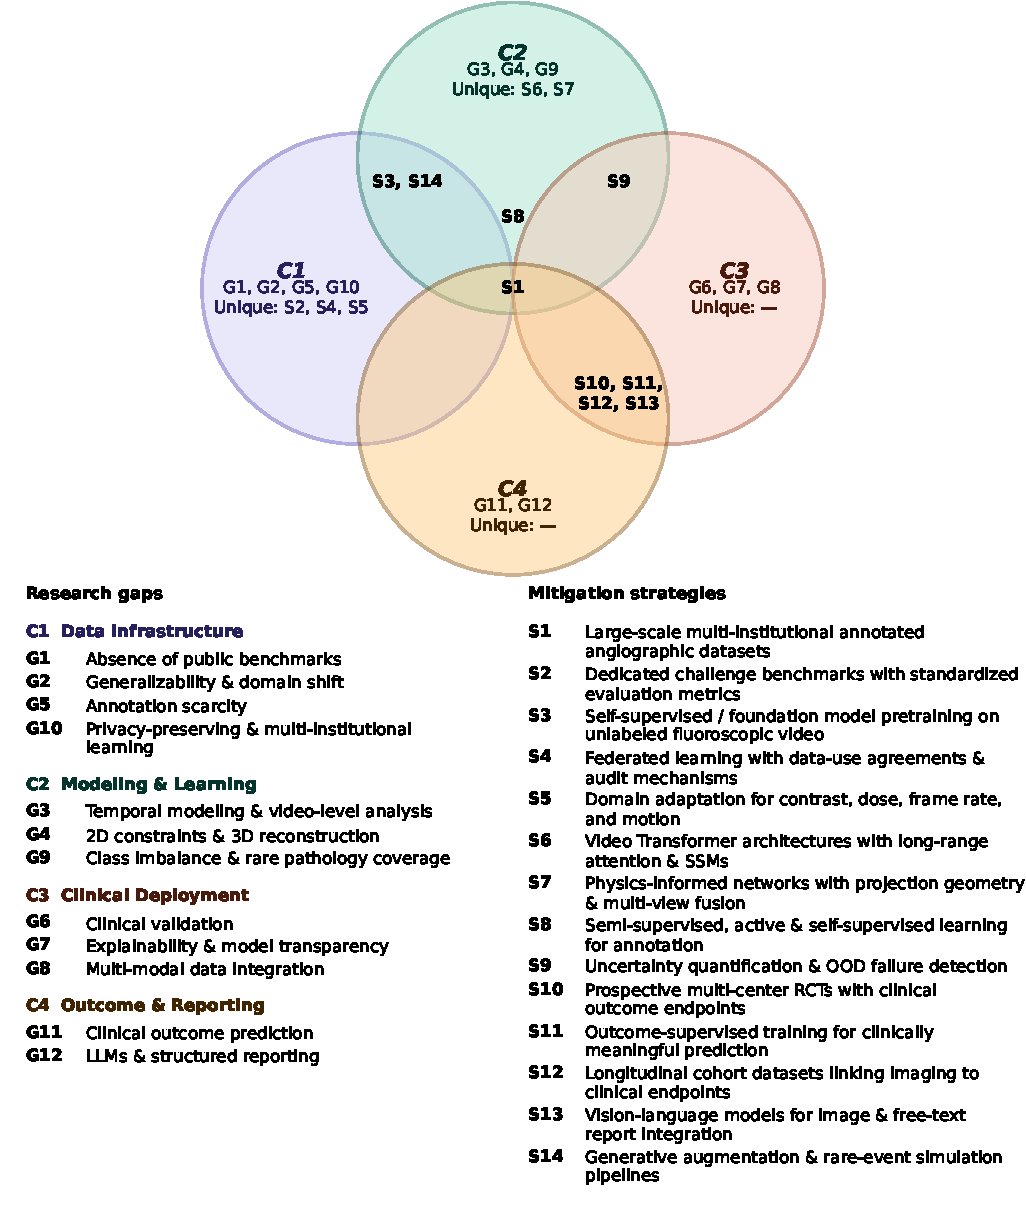
\includegraphics[height=11.5cm,width=\textwidth]{figs/venn_diagram.pdf}
  \caption{Thematic clustering of research gaps and mitigation strategies identified in the systematic review of AI-based angiographic and fluoroscopic image analysis. The four overlapping circles represent thematic clusters: \textbf{C1 --- Data Infrastructure} (gaps G1, G2, G10; lavender); \textbf{C2 --- Modeling \& Learning} (gaps G3, G4, G5, G9; green); \textbf{C3 --- Clinical Deployment} (gaps G6, G7, G8; salmon); and \textbf{C4 --- Outcome \& Reporting} (gaps G11, G12; amber). Overlap regions carry the strategy codes (S1--S14) shared across the intersecting clusters: the C1--C2 intersection is addressed by S1 (large-scale multi-institutional datasets); the C2--C3 intersection by S8 (annotation-efficient learning) and S9 (uncertainty quantification); and the C3--C4 intersection by S10--S13 (prospective
  trials, outcome-supervised training, longitudinal cohort datasets, and
  vision-language integration). Strategy S1 also is at the centre of
  all four clusters, reflecting its foundational role across every
  thematic domain. Strategies unique to each cluster are listed within
  the respective circle: C1 uniquely requires S2 (challenge benchmarks),
  S4 (federated learning), and S5 (domain adaptation); C2 uniquely
  requires S3 (foundation model pretraining), S6 (video Transformer
  architectures), S7 (physics-informed networks), and S14 (generative
  augmentation). Dashes (---) denote cluster intersections for which no
  shared strategy was identified across the reviewed literature. Gap and
  strategy codes correspond to the identifiers used throughout
  Table~\ref{tab:research_gaps} and the accompanying narrative.}
  \label{fig:venn_gaps}
\end{figure*}

Twelve research gaps identified across the 194 included studies can be organized into four thematic clusters that reflect the structural
layers at which the current literature exhibits shortcomings (Figure~\ref{fig:venn_gaps}). The first cluster, \textit{Data
Infrastructure} (C1), encompasses gaps in dataset size, public
availability, cross-institutional generalizability, and
privacy-preserving learning (G1, G2, G10); these are upstream constraints
whose resolution is a precondition for progress in every other area. The
second cluster, \textit{Modeling \& Learning} (C2), groups the
methodological gaps that limit what can be done even when data are
available: inadequate temporal modeling of angiographic video sequences,
the restriction to 2D projections, annotation scarcity, and class
imbalance (G3, G4, G5, G9). The third cluster, \textit{Clinical
Deployment} (C3), captures the gap between technical feasibility and
clinical readiness: the near-total absence of prospective validation, the
lack of model explainability, and the failure to integrate complementary
imaging modalities (G6, G7, G8). The fourth cluster, \textit{Outcome \&
Reporting} (C4), addresses the most distal translation gap: the
disconnection between imaging-level task performance and the clinical
outcome prediction and structured reporting capabilities that would make
AI tools genuinely useful at the point of care (G11, G12). As shown in
Figure~\ref{fig:venn_gaps}, these clusters are not independent. The
C1--C2 intersection is bridged by the construction of large-scale
annotated datasets (S1), which simultaneously enables better model
training and reduces annotation burden. The C2--C3 intersection is
addressed by annotation-efficient learning strategies (S8) and
uncertainty quantification frameworks (S9), both of which are
prerequisites for safe clinical deployment of models trained under data
constraints. The C3--C4 intersection is where prospective trial design
(S10), outcome-supervised training (S11), longitudinal cohort datasets
(S12), and vision-language integration (S13) converge, reflecting the
interdependence of clinical validation and outcome reporting. Strategy S1
occupies the centre of all four clusters because the availability of
large, diverse, well-annotated angiographic datasets is the single
intervention with the broadest leverage across every identified gap. Table~\ref{tab:research_gaps} details the evidence base for each gap and articulates
the corresponding future research directions.

% A systematic analysis of the limitations and future work directions
% reported across the 194 included studies reveals a set of recurring,
% structural deficiencies in the current state of artificial intelligence
% applied to angiographic and fluoroscopic imaging. Table~\ref{tab:research_gaps}
% consolidates the identified gaps and the corresponding proposed directions
% across twelve thematic research areas.

% ============================================================
% TABLE — portrait, no landscape required
% \small reduces font to ~8.5pt, giving ~15% more horizontal room.
% Column widths: 2.5 + 6.5 + 6.5 = 15.5 cm (fits A4 with 2 cm margins).
% \clearpage + \onecolumn escape two-column mode for longtable.
% \clearpage + \twocolumn restore it cleanly afterward.
% ============================================================
\clearpage
\onecolumn
\small

\begin{longtable}{>{\raggedright\arraybackslash}p{2.5cm}
                  >{\raggedright\arraybackslash}p{6.5cm}
                  >{\raggedright\arraybackslash}p{6.5cm}}

\caption{Evidence-driven research gaps and proposed future directions
identified from the systematic review of AI-based angiographic and
fluoroscopic image analysis.}
\label{tab:research_gaps} \\

\toprule
\textbf{Research Gaps} & \textbf{Evidence from the Literature} &
\textbf{Mitigation Strategies} \\
\midrule
\endfirsthead

\multicolumn{3}{c}{\tablename~\thetable{} --
  \textit{continued from previous page}} \\
\toprule
\textbf{Research Area} & \textbf{Identified Gap} &
\textbf{Mitigation Strategies} \\
\midrule
\endhead

\midrule
\multicolumn{3}{r}{\textit{Continued on next page}} \\
\endfoot

\bottomrule
\endlastfoot

% ---- Row 1 ----
\textbf{G1:} Absence of Public Benchmarks
&
\tabitem Small, private, single-center datasets dominate; most cohorts contain fewer than 200 patients \cite{ref20,ref24,ref41,ref45,ref71,ref72,ref78,ref79,ref85,ref86}.\newline
\tabitem No publicly available, annotated benchmark dataset specific to angiographic imaging exists \cite{ref4,ref15,ref27,ref34,ref50,ref56,ref63}.\newline
\tabitem Absence of shared benchmarks makes cross-study comparison practically impossible \cite{ref6,ref11,ref26,ref33,ref38,ref49,ref57,ref58,ref87,ref97,ref98,ref99}.\newline
\tabitem Inconsistent evaluation protocols prevent measurement of field-wide progress \cite{ref1,ref65,ref89}.
&
\tabitem Construct and release large-scale multi-institutional angiographic datasets with standardized pixel-level annotations and defined train/test splits \cite{ref15,ref29,ref63,ref75,ref94}.\newline
\tabitem Organize dedicated challenge benchmarks modeled on established medical image segmentation competitions \cite{ref2,ref39}.\newline
\tabitem Mandate inter-rater reliability protocols in annotation guidelines to ensure label quality \cite{ref19}.\newline
\tabitem Define standard evaluation metrics and phantom-versus-patient evaluation subsets \cite{ref29}.
\\
\dashedrule

% ---- Row 2 ----
\textbf{G2:} Generalizability \& Domain Shift
&
\tabitem Models trained on a single vendor or acquisition protocol consistently fail to transfer to external settings \cite{ref5,ref9,ref10,ref15,ref27,ref29,ref38,ref83,ref93}.\newline
\tabitem Domain shift between synthetic training data and real clinical images remains unresolved \cite{ref52,ref64,ref74}.\newline
\tabitem Methods validated on coronary angiography degrade when applied to cerebral, renal, or peripheral vasculature \cite{ref16,ref40,ref56,ref62,ref63,ref65,ref75,ref81}.\newline
\tabitem Multi-center heterogeneity in frame rate, contrast dosing, and radiation settings is rarely addressed \cite{ref14,ref17,ref19,ref23,ref25,ref51,ref92,ref95}.
&
\tabitem Treat external multi-institutional validation as a required component, not an optional addition \cite{ref15,ref19,ref75}.\newline
\tabitem Develop domain adaptation methods tailored to variable contrast concentration, dose, frame rate, and motion profiles \cite{ref17,ref64}.\newline
\tabitem Extend personalized federated learning frameworks to accommodate non-identical cross-center data distributions \cite{ref19}.\newline
\tabitem Establish domain shift benchmarks to quantify performance degradation across imaging vendors \cite{ref5,ref64}.
\\
\dashedrule

% ---- Row 3 ----
\textbf{G3:} Temporal Modeling \& Video-Level Analysis
&
\tabitem Most methods treat each frame as an independent 2D image, discarding hemodynamic flow and contrast propagation dynamics \cite{ref31,ref50,ref52,ref58,ref65,ref93}.\newline
\tabitem Temporal models are typically restricted to short fixed-length clips, not full variable-length sequences \cite{ref10,ref34,ref36,ref67}.\newline
\tabitem Procedural phase transitions during interventional procedures are not explicitly modeled \cite{ref25,ref48,ref65}.\newline
\tabitem Respiratory and cardiac motion are treated as noise rather than informative temporal signals \cite{ref18,ref77,ref96}.
&
\tabitem Develop architectures that model the complete temporal structure of angiographic acquisitions, including mask, injection, and washout phases \cite{ref32,ref34,ref66}.\newline
\tabitem Evaluate video Transformer architectures with long-range attention and state-space models for efficient long-sequence processing \cite{ref25,ref66,ref93}.\newline
\tabitem Explore temporal self-supervised pretraining on large archives of unannotated fluoroscopic video \cite{ref18}.\newline
\tabitem Incorporate explicit hemodynamic priors into temporal model design \cite{ref77}.
\\
\dashedrule

% ---- Row 4 ----
\textbf{G4:} 2D Constraints \& 3D Reconstruction
&
\tabitem Angiographic projections collapse 3D vascular anatomy, introducing foreshortening, vessel overlap, and depth loss \cite{ref1,ref31,ref35,ref40,ref66}.\newline
\tabitem The vast majority of methods operate exclusively on single-plane 2D projections \cite{ref23,ref33,ref44,ref62}.\newline
\tabitem Robust 3D reconstruction from monoplane or biplane projections under intraoperative time constraints remains unsolved \cite{ref43,ref54,ref55,ref90}.\newline
\tabitem 2D/3D registration accuracy is insufficient for routine intraoperative use \cite{ref55,ref82}.
&
\tabitem Develop multi-view learning architectures that fuse information across projection angles \cite{ref23,ref66,ref90}.\newline
\tabitem Investigate physics-informed networks incorporating known projection geometry and contrast agent kinetics \cite{ref43,ref55}.\newline
\tabitem Leverage rotational angiographic acquisitions for temporally informed 3D reconstruction \cite{ref54,ref82}.\newline
\tabitem Systematically combine intraoperative cone-beam CT with fluoroscopic AI pipelines to provide 3D context \cite{ref21}.
\\
\dashedrule

% ---- Row 5 ----
\textbf{G5:} Annotation Scarcity \& Annotation-Efficient Learning
&
\tabitem Manual annotation requires substantial physician time and specialized expertise per labeled study \cite{ref2,ref13,ref34,ref67,ref87,ref97,ref98,ref99}.\newline
\tabitem Annotation is subject to significant intra- and inter-observer variability, rarely quantified in included studies \cite{ref4,ref11,ref46,ref56,ref58}.\newline
\tabitem Synthetic data generation partially addresses scarcity, but synthetic-to-real domain gaps persist \cite{ref52,ref64,ref74,ref98}.\newline
\tabitem Semi-supervised and self-supervised methods are underrepresented across angiographic analysis tasks \cite{ref18,ref49}.
&
\tabitem Systematically evaluate semi-supervised, self-supervised, and active learning strategies with explicit performance-versus-label-count analysis \cite{ref2,ref49,ref74}.\newline
\tabitem Pursue foundation model pretraining on large archives of unlabeled fluoroscopic video \cite{ref18}.\newline
\tabitem Validate generative data augmentation methods informed by realistic vascular anatomy models and imaging physics \cite{ref52,ref64}.\newline
\tabitem Develop annotation tools that integrate uncertainty estimation to prioritize the most informative cases for expert labeling \cite{ref46}.
\\
\dashedrule

% ---- Row 6 ----
\textbf{G6:} Prospective Clinical Validation \& Outcome Assessment
&
\tabitem Nearly all included studies rely on retrospective analysis of previously acquired images \cite{ref14,ref26,ref42,ref53,ref59,ref61,ref76,ref84,ref91}.\newline
\tabitem Prospective validation in live clinical settings is almost entirely absent from the literature \cite{ref1,ref7,ref16,ref25,ref49,ref51,ref65}.\newline
\tabitem Retrospective evaluation cannot measure the effect of AI outputs on physician behavior or patient outcomes \cite{ref37,ref68,ref70}.\newline
\tabitem Demonstrated technical performance does not establish clinical value or cost-effectiveness \cite{ref53,ref65}.
&
\tabitem Design prospective clinical evaluation frameworks in collaboration between AI researchers and clinicians from the outset \cite{ref14,ref42}.\newline
\tabitem Pursue randomized controlled trials comparing outcomes under standard-of-care versus AI-assisted decision-making \cite{ref25,ref76}.\newline
\tabitem Engage regulatory bodies early to define the evidence standards required for clinical deployment \cite{ref39,ref59}.\newline
\tabitem Develop AI interface designs that integrate model outputs into existing workflow without adding cognitive burden \cite{ref84}.
\\
\dashedrule

% ---- Row 7 ----
\textbf{G7:} Explainability \& Model Transparency
&
\tabitem Most deep learning models produce predictions without clinically interpretable justification \cite{ref14,ref65}.\newline
\tabitem Existing attention visualization approaches provide limited mechanistic insight \cite{ref68,ref89}.\newline
\tabitem Silent failure modes in out-of-distribution inputs are a particular concern for patient safety \cite{ref25}.\newline
\tabitem Regulatory and clinical trust requirements are not satisfied by aggregate performance metrics alone \cite{ref14,ref89}.
&
\tabitem Treat uncertainty quantification as a core design requirement, communicating confidence alongside every prediction \cite{ref14,ref25}.\newline
\tabitem Develop failure detection systems that flag out-of-distribution inputs for mandatory human review \cite{ref25,ref68}.\newline
\tabitem Design intermediate representations aligned with clinically meaningful anatomical and hemodynamic concepts \cite{ref68}.\newline
\tabitem Evaluate whether explainability outputs demonstrably improve clinical decision-making in prospective user studies \cite{ref89}.
\\
\dashedrule

% ---- Row 8 ----
\textbf{G8:} Multi-Modal Data Integration
&
\tabitem Studies predominantly process angiographic images in isolation, discarding complementary clinical data \cite{ref16,ref32,ref62}.\newline
\tabitem Pressure wire measurements, IVUS, OCT, CTA, ECG, and laboratory biomarkers are routinely available but unused \cite{ref30,ref46,ref69,ref81,ref91}.\newline
\tabitem Missing modalities at inference time, common in clinical practice, are rarely addressed \cite{ref25,ref84}.\newline
\tabitem Longitudinal multi-modal datasets linking intraoperative imaging to procedural outcomes are essentially absent \cite{ref21}.
&
\tabitem Develop architectures capable of fusing imaging, hemodynamic, and structured clinical data with explicit handling of missing modalities \cite{ref25,ref32}.\newline
\tabitem Construct longitudinal multi-modal cohort datasets linking angiographic sequences to post-procedural outcomes \cite{ref21,ref91}.\newline
\tabitem Explore vision-language model architectures for integrating free-text clinical notes with imaging features \cite{ref30}.\newline
\tabitem Define outcome-oriented multi-modal training objectives that directly optimize for clinically meaningful predictions \cite{ref46,ref69}.
\\
\dashedrule

% ---- Row 9 ----
\textbf{G9:} Class Imbalance \& Rare Pathology Coverage
&
\tabitem Rare events such as vessel perforation, intracranial aneurysm, and gastrointestinal bleeding are severely underrepresented \cite{ref20,ref21,ref80}.\newline
\tabitem Standard training objectives produce models biased toward majority classes with poor sensitivity for critical minority cases \cite{ref4,ref25,ref57,ref65,ref79,ref89}.\newline
\tabitem Rare anatomical variants and complex lesion morphologies are systematically excluded from study cohorts \cite{ref47,ref50,ref87}.\newline
\tabitem Aggregate performance metrics obscure minority-class failure, masking clinically important shortcomings \cite{ref80,ref89}.
&
\tabitem Systematically evaluate oversampling, cost-sensitive learning, hard negative mining, and generative augmentation across imbalance ratios \cite{ref4,ref80}.\newline
\tabitem Explicitly target underrepresented pathology types in dataset construction rather than excluding them \cite{ref20}.\newline
\tabitem Mandate stratified reporting of performance metrics for rare classes alongside aggregate figures \cite{ref80}.\newline
\tabitem Develop rare-event simulation pipelines for synthetic augmentation of clinically critical minority cases \cite{ref80}.
\\
\dashedrule

% ---- Row 10 ----
\textbf{G10:} Privacy-Preserving \& Multi-Institutional Learning
&
\tabitem Patient privacy regulations and data governance barriers prevent centralization of large angiographic datasets \cite{ref14,ref15,ref75}.\newline
\tabitem Federated learning for angiographic analysis is barely represented in the reviewed literature; only one study explicitly adopts this framework \cite{ref19}.\newline
\tabitem Non-identical data distributions across institutions complicate federated model training \cite{ref19,ref92}.\newline
\tabitem Auditability and accountability requirements for federated clinical AI systems are unaddressed \cite{ref14}.
&
\tabitem Develop federated learning frameworks specifically tailored to large angiographic video inputs with efficient communication protocols \cite{ref19}.\newline
\tabitem Evaluate differential privacy and secure multi-party computation approaches for their impact on model utility \cite{ref19}.\newline
\tabitem Establish standardized data use agreements and federated audit mechanisms for cross-institutional AI training \cite{ref15,ref19}.\newline
\tabitem Benchmark personalized federated approaches against centralized baselines as a function of institutional data heterogeneity \cite{ref19}.
\\
\dashedrule

% ---- Row 11 ----
\textbf{G11}: Imaging Biomarkers \& Clinical Outcome Prediction
&
\tabitem Most methods focus on intermediate imaging tasks rather than on direct clinical outcome prediction \cite{ref1,ref14,ref25,ref69,ref84}.\newline
\tabitem Demonstrating detection or segmentation accuracy does not establish impact on revascularization decisions or survival \cite{ref42,ref59,ref91}.\newline
\tabitem Longitudinal cohort designs linking imaging findings to follow-up clinical endpoints are largely absent \cite{ref71,ref72,ref76}.\newline
\tabitem Outcome-supervised training objectives have not been systematically explored in the angiographic domain \cite{ref84,ref91}.
&
\tabitem Construct longitudinal datasets linking intraoperative angiographic images to post-procedural endpoints including re-intervention rates and mortality \cite{ref42,ref76}.\newline
\tabitem Develop outcome-supervised training objectives that directly optimize for clinically meaningful event prediction \cite{ref14,ref84}.\newline
\tabitem Apply imaging biomarker discovery workflows combining feature extraction with survival and outcome modeling \cite{ref59,ref71,ref72}.\newline
\tabitem Integrate procedural databases and electronic health record data with angiographic image archives to enable outcome-linked training \cite{ref84,ref91}.
\\
\dashedrule

% ---- Row 12 ----
\textbf{G12}: Large Language Models \& Structured Reporting
&
\tabitem LLM application to angiographic reporting and clinical knowledge integration is almost entirely unexplored; only one study in this review addresses this area \cite{ref73}.\newline
\tabitem Free-text angiographic reports contain rich structured information routinely discarded in downstream analyses \cite{ref73}.\newline
\tabitem The only included study on LLM-based report structuring is geographically restricted to Korean institutions and relies on proprietary models, limiting reproducibility \cite{ref73}.\newline
\tabitem Multimodal vision-language models for integrated image-and-report reasoning have not been evaluated in this domain \cite{ref73}.
&
\tabitem Evaluate open-source LLMs and vision-language models for angiographic report structuring, finding extraction, and downstream decision support \cite{ref73}.\newline
\tabitem Develop end-to-end pipelines that integrate structured imaging outputs with natural language generation for automated report synthesis \cite{ref73}.\newline
\tabitem Construct standardized angiographic reporting ontologies to provide a shared vocabulary for cross-institutional NLP model training \cite{ref73}.\newline
\tabitem Benchmark open-source models against proprietary baselines on diverse international angiographic report corpora \cite{ref73}.
\\

\end{longtable}

\subsection{Toward an Actionable Roadmap}
\label{sec:actionable_roadmap}

While Table~\ref{tab:research_gaps} documents the evidence base and candidate mitigation strategies for each gap, it does not by itself prioritize where the field should act first or specify how progress could be measured. Table~\ref{tab:cbm_roadmap} distills this analysis into a compact, actionable roadmap: for each gap, it reports the number of included studies documenting the gap in the literature (Evidence Count, computed directly from the citations underlying Table~\ref{tab:research_gaps}), the clinical risk of leaving the gap unaddressed, the corresponding computational opportunity, and a concrete benchmark or evaluation recommendation that would make progress on the gap measurable. Gaps with the largest evidence bases (G1, G2, G6) represent the most extensively documented structural barriers in the current literature, whereas gaps with a narrow evidence base (G7, G10, G12) reflect emerging but still underexplored directions.

\footnotesize
\begin{longtable}{>{\raggedright\arraybackslash}p{2.1cm}
                  >{\centering\arraybackslash}p{1.1cm}
                  >{\raggedright\arraybackslash}p{4.1cm}
                  >{\raggedright\arraybackslash}p{4.1cm}
                  >{\raggedright\arraybackslash}p{4.3cm}}

\caption{CBM-facing actionable roadmap synthesizing each research gap identified in Table~\ref{tab:research_gaps} into clinical risk, computational opportunity, and a concrete benchmark or evaluation recommendation. Evidence Count is the number of distinct included studies cited as documenting each gap in Table~\ref{tab:research_gaps}.}
\label{tab:cbm_roadmap} \\

\toprule
\textbf{Gap} & \textbf{Evid.\ Count} & \textbf{Clinical Risk} & \textbf{Computational Opportunity} & \textbf{Benchmark / Evaluation Recommendation} \\
\midrule
\endfirsthead

\multicolumn{5}{c}{\tablename~\thetable{} -- \textit{continued from previous page}} \\
\toprule
\textbf{Gap} & \textbf{Evid.\ Count} & \textbf{Clinical Risk} & \textbf{Computational Opportunity} & \textbf{Benchmark / Evaluation Recommendation} \\
\midrule
\endhead

\midrule
\multicolumn{5}{r}{\textit{Continued on next page}} \\
\endfoot

\bottomrule
\endlastfoot

\textbf{G1} Absence of Public Benchmarks & 32 &
Reported performance cannot be verified to generalize beyond the originating institution before deployment, risking undetected failure in new clinical settings. &
Large-scale, standardized, publicly released multi-institutional datasets with defined train/test splits. &
Organize a public challenge benchmark with standardized metrics and phantom-versus-patient evaluation subsets. \\
\dashedrule

\textbf{G2} Generalizability \& Domain Shift & 28 &
Models validated at a single site, vendor, or vascular territory may silently degrade elsewhere, producing unreliable outputs during patient care without warning. &
Domain adaptation and personalized federated learning tailored to cross-vendor, cross-protocol, and cross-territory variation. &
Require external multi-institutional validation and report a domain-shift benchmark quantifying degradation across imaging vendors. \\
\dashedrule

\textbf{G3} Temporal Modeling \& Video-Level Analysis & 15 &
Discarding hemodynamic flow and contrast-propagation dynamics risks missing clinically important temporal signals a frame-independent model cannot detect. &
Video-transformer and state-space architectures modeling full acquisition phases (mask, injection, washout) with hemodynamic priors. &
Evaluate on full variable-length real acquisitions with metrics scoring temporal fidelity, not accuracy on short fixed-length clips alone. \\
\dashedrule

\textbf{G4} 2D Constraints \& 3D Reconstruction & 14 &
Foreshortening, vessel overlap, and depth loss from monoplane 2D projections can cause missed or mis-measured lesions during intraoperative decisions. &
Multi-view and physics-informed 3D reconstruction from mono-/biplane or rotational angiographic acquisitions. &
Standardized 2D/3D registration accuracy benchmark evaluated under intraoperative time constraints. \\
\dashedrule

\textbf{G5} Annotation Scarcity \& Annotation-Efficient Learning & 18 &
Reliance on scarce expert annotation with unquantified inter-observer variability threatens label reliability for safety-critical model training. &
Semi-/self-supervised and active learning, foundation-model pretraining on large archives of unlabeled fluoroscopic video. &
Report performance-versus-label-count curves for each annotation-efficient method, rather than accuracy at a single fixed label budget. \\
\dashedrule

\textbf{G6} Prospective Clinical Validation \& Outcome Assessment & 19 &
Because almost no studies validate prospectively, there is no evidence these models change physician behavior or patient outcomes in live care. &
Prospective evaluation frameworks and outcome-supervised training designed jointly with clinicians from the outset. &
Randomized controlled trials comparing standard-of-care versus AI-assisted decision-making as the evaluation standard. \\
\dashedrule

\textbf{G7} Explainability \& Model Transparency & 5 &
Predictions without interpretable justification, and unflagged out-of-distribution failures, can silently mislead clinicians and undermine patient safety. &
Uncertainty quantification and failure-detection systems flagging out-of-distribution inputs for mandatory human review. &
Prospective user studies testing whether explainability outputs measurably improve clinical decision-making, not qualitative attention maps alone. \\
\dashedrule

\textbf{G8} Multi-Modal Data Integration & 11 &
Ignoring routinely available complementary data (IVUS, OCT, ECG, labs) means models may miss clinically decisive information a clinician would normally use. &
Fusion architectures with explicit handling of missing modalities; vision-language integration of free-text clinical notes. &
Outcome-oriented multi-modal benchmarks that explicitly test performance under missing-modality conditions. \\
\dashedrule

\textbf{G9} Class Imbalance \& Rare Pathology Coverage & 12 &
Models biased toward majority classes may have poor sensitivity for rare but critical events (e.g., perforation, aneurysm) -- precisely the cases where failure is most dangerous. &
Cost-sensitive learning, hard negative mining, and rare-event simulation or generative augmentation. &
Mandate stratified per-class sensitivity reporting for rare pathologies alongside aggregate accuracy metrics. \\
\dashedrule

\textbf{G10} Privacy-Preserving \& Multi-Institutional Learning & 5 &
Data governance barriers blocking multi-institutional pooling constrain how representative and safe models can be before wide deployment. &
Federated learning frameworks and differential privacy / secure multi-party computation for angiographic video. &
Benchmark personalized federated approaches against centralized baselines as a function of institutional data heterogeneity. \\
\dashedrule

\textbf{G11} Imaging Biomarkers \& Clinical Outcome Prediction & 11 &
Strong segmentation or detection accuracy does not establish that a model improves revascularization decisions or survival, so technical success may not translate to patient benefit. &
Outcome-supervised training objectives and imaging-biomarker discovery combined with survival modeling. &
Longitudinal cohort evaluation linking imaging-derived predictions to real clinical endpoints (re-intervention rate, mortality), not intermediate task metrics alone. \\
\dashedrule

\textbf{G12} Large Language Models \& Structured Reporting & 1 &
With only one included study (geographically and model-restricted), there is essentially no evidence base for LLM-assisted angiographic reporting, so its safety and reliability for clinical use is unknown. &
Open-source LLM and vision-language pipelines for angiographic report structuring and finding extraction. &
Benchmark open-source against proprietary models on diverse international angiographic report corpora using a standardized reporting ontology. \\

\end{longtable}
\normalsize

\clearpage
\twocolumn



